\chapter{Introduction}

\label{sec:interfaces}

\begin{figure}
\center{
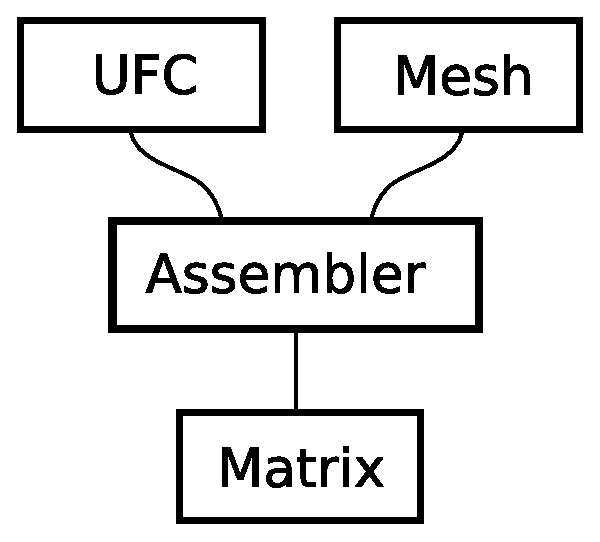
\includegraphics[width=6cm]{eps/ufcfig.eps}
\caption{Main components in a finite element assembly application.}
\label{fig:ufc-assembler}
}
\end{figure}

Large parts of a finite element program are similar from problem to
problem and can therefore be coded as a general, reusable library.
Mesh data structures, linear algebra and finite element assembly are
examples of operations that are naturally coded in a
problem-independent way and made available in reusable
libraries~\cite{logg:www:03,Sundance,dealII,FEMLAB,Cactus,UG,Kaskade,Overture,PETSc,Trilinos,www:Diffpack}.
However, some parts of a finite element program are difficult to code
in a problem-independent way. In particular, this includes the
evaluation of the \emph{element tensor} (the ``element stiffness
matrix''), that is, the evaluation of the local contribution from a
finite element to a global sparse global sparse tensor (the
``stiffness matrix'') representing a discretized differential
operator. These parts must thus be implemented by the application
programmer for each specific combination of differential equation and
discretization (finite element spaces).

However, domain-specific compilers such as FFC~\cite{www:ffc,other}
and SyFi~\cite{www:syfi,other} make it possible to automatically
generate the code for the evaluation of the element tensor. These
\emph{form compilers} accept as input a high-level description of a
finite element variational form and generates low-level code code for
efficient evaluation of the element tensor and associated quantities.
It thus becomes important to specify the \emph{interface} between form
compilers and finite element assemblers such that the code generated
by FFC, SyFi and other form compilers can be used to assemble finite
element matrices and vectors (and in general tensors).

UFC (Unified Form-assembly Code) is a unified framework for finite
element assembly in the form of a fixed interface for the code
generated by form compilers. It consists of a single header
\texttt{ufc.h} that specifies a C++ interface that must be implemented
by UFC-compliant form compilers. Both FFC (since version 0.4.0) and
SyFi (since version x.y.z) generate code that complies with the UFC
specification. Thus, code generated by FFC and SyFi may be used
interchangeably by any UFC-based finite element assemblers, such as
DOLFIN~\cite{www:dolfin,other}.
